\documentclass[12pt, a4paper]{article}
\usepackage{iftex}
\ifPDFTeX
  \usepackage{cmap}
  \usepackage[T2A]{fontenc}
  \usepackage[utf8]{inputenc}
  \usepackage{tempora}
\else
  \usepackage{fontspec}
  \IfFontExistsTF{Times New Roman}
    {\setmainfont{Times New Roman}}
    {\setmainfont{CMU Serif}}
  \IfFontExistsTF{Consolas}
    {\setmonofont{Consolas}[Scale=MatchLowercase]}
    {\IfFontExistsTF{Courier New}
      {\setmonofont{Courier New}}
      {\setmonofont{CMU Typewriter Text}}}
\fi
\usepackage[english,russian]{babel}

\usepackage[a4paper, margin=2.54cm]{geometry}
\setlength{\parindent}{0pt}
\setlength{\parskip}{4pt plus 1pt}
\frenchspacing
\raggedbottom

\usepackage{titlesec}
\setcounter{secnumdepth}{0}
\titleformat{\section}{\large\bfseries}{}{0pt}{}
\titleformat{\subsection}{\normalsize\bfseries}{}{0pt}{}
\titlespacing*{\section}{0pt}{14pt plus 4pt minus 2pt}{4pt plus 2pt}
\titlespacing*{\subsection}{0pt}{10pt plus 2pt minus 2pt}{3pt plus 1pt}

\usepackage[table]{xcolor}
\usepackage{graphicx}
\usepackage{tabularx}
\usepackage{float}
\usepackage{caption}
\DeclareCaptionLabelSeparator{spacedemdash}{~--- }
\captionsetup{labelsep=spacedemdash, font=small, singlelinecheck=false, justification=raggedright}
\captionsetup[table]{position=top, skip=4pt}
\DeclareCaptionType[fileext=lol]{listing}[Листинг][Листинги]
\captionsetup[listing]{position=top, skip=4pt, hypcap=false}
\addto\captionsrussian{\renewcommand{\figurename}{Рисунок}\renewcommand{\tablename}{Таблица}}
\newcommand{\thead}[1]{\multicolumn{1}{|c|}{\cellcolor{gray!20}\textbf{#1}}}
\newcolumntype{L}{>{\raggedright\arraybackslash}X}
\newcolumntype{P}[1]{>{\raggedright\arraybackslash}p{#1}}

\usepackage{fvextra}
\usepackage{needspace}
\fvset{breaklines=true, breakanywhere=true,
       frame=leftline, framerule=1.5pt, framesep=6pt,
       rulecolor=\color{gray!60}, xleftmargin=4pt}
\DefineVerbatimEnvironment{code}{Verbatim}{fontsize=\small}
\DefineVerbatimEnvironment{terminal}{Verbatim}{fontsize=\footnotesize}
\newcommand{\inputterminal}[2][]{\VerbatimInput[fontsize=\footnotesize,#1]{#2}}
\ifPDFTeX
  \usepackage{listingsutf8}
  \lstset{inputencoding=utf8/cp1251, basicstyle=\fontencoding{T2A}\selectfont\ttfamily\small,
          breaklines=true, breakatwhitespace=false, columns=fullflexible,
          keepspaces=true, showstringspaces=false, frame=leftline,
          framerule=1.5pt, framesep=6pt, xleftmargin=4pt,
          rulecolor=\color{gray!60}}
  \newcommand{\inputcode}[2][]{\lstinputlisting[#1]{#2}}
  \newcommand{\inputappendixcode}[2][]{\lstinputlisting[basicstyle=\linespread{0.90}\fontencoding{T2A}\selectfont\ttfamily\footnotesize,#1]{#2}}
\else
  \newcommand{\inputcode}[2][]{\VerbatimInput[fontsize=\small,#1]{#2}}
  \newcommand{\inputappendixcode}[2][]{\VerbatimInput[fontsize=\footnotesize,baselinestretch=0.90,#1]{#2}}
\fi
\newenvironment{listingblock}[1]
  {\Needspace{8\baselineskip}\par\medskip\captionof{listing}{#1}\nopagebreak\vspace{-\topsep}\vspace{-\parskip}}
  {\par}

\newcounter{appendixno}
\newcommand{\appendixsection}[2]{\clearpage\section{Приложение #1. #2}\stepcounter{appendixno}\setcounter{listing}{0}\renewcommand{\thelisting}{#1.\arabic{listing}}\renewcommand{\theHlisting}{app\arabic{appendixno}.\arabic{listing}}}

\usepackage[hidelinks]{hyperref}
\usepackage{xurl}

\newcommand{\hint}[1]{\leavevmode{\color{gray}\itshape #1}}
\newcommand{\placeholder}[2][4.5cm]{\fbox{\parbox[c][#1][c]{0.95\linewidth}{\centering\hint{#2}}}}


\newcommand{\ReportLab}{3}
\newcommand{\ReportStudent}{Новак Дмитрий Евгеньевич}
\newcommand{\ReportGroup}{М8О-201БВ-25}
\newcommand{\ReportTeacher}{Миронов Евгений Сергеевич}
\newcommand{\ReportDate}{15.10.2026}
\newcommand{\ReportYear}{2026}
\newcommand{\ReportCourse}{Операционные системы и архитектура компьютера}

\begin{document}
% Титульный лист. Данные берутся из команд \Report... в report.tex.
\begin{titlepage}
  \centering\large

  МОСКОВСКИЙ АВИАЦИОННЫЙ ИНСТИТУТ\\
  (НАЦИОНАЛЬНЫЙ ИССЛЕДОВАТЕЛЬСКИЙ УНИВЕРСИТЕТ)\par
  \vspace{18pt}
  Институт №8 «Компьютерные науки и прикладная математика»\\
  Кафедра 806 «Вычислительная математика и программирование»\par

  \vspace{\stretch{1.2}}

  {\bfseries Лабораторная работа №\,\ReportLab{} по курсу\\
  «\ReportCourse»\par}

  \vspace{\stretch{1.6}}

  \begin{flushright}
    \begin{tabular}{r@{\hspace{0.6em}}l}
      Выполнил:      & \ReportStudent \\[2pt]
      Группа:        & \ReportGroup   \\[2pt]
      Преподаватель: & \ReportTeacher \\[2pt]
      Дата:          & \ReportDate    \\[2pt]
      Оценка:        & \rule[-2pt]{4.2cm}{0.4pt} \\
    \end{tabular}
  \end{flushright}

  \vspace{\stretch{1}}

  Москва, \ReportYear
\end{titlepage}
\setcounter{page}{2}


\section{Условие}

\textbf{Цель работы:} получить практические навыки создания потоков и
синхронизации между ними, исследовать ускорение параллельного алгоритма.

\textbf{Задание:} написать на языке C многопоточную программу. Максимальное
количество одновременно работающих потоков задаётся ключом запуска. Нужно
показать число потоков средствами ОС и исследовать влияние размера входных
данных и числа потоков на ускорение и эффективность.

\textbf{Вариант 3:} сортировка массива целых чисел параллельным алгоритмом
слияния.

\section{Метод решения}

Программа читает целые числа из файла в массив. Сортировка выполняется
итеративно: на проходе с шириной $w$ сливаются соседние отсортированные
отрезки длиной не более $w$, затем $w$ удваивается. Каждый поток получает
независимые пары отрезков по циклическому распределению. Потоки читают из
одного массива и записывают в непересекающиеся участки второго. После
завершения всех слияний прохода барьер позволяет одному потоку поменять
указатели на массивы. Второй барьер гарантирует, что остальные увидят
новые указатели до следующего прохода.

Главный поток участвует в сортировке, поэтому при ключе
\texttt{--threads p} создаётся не более $p-1$ дополнительных потоков.
Если элементов меньше $p$, используются только необходимые потоки.
Алгоритм требует $O(n\log n)$ сравнений и $O(n)$ дополнительной памяти.
Слияние на одном проходе делится между потоками без блокировок на элементах
массива. На последних проходах пар мало, поэтому число одновременно
занятых вычислениями потоков может быть меньше заданного предела.

\section{Описание программы}

\subsection{Структура файлов}

\begin{table}[H]
  \caption{Основные файлы лабораторной работы}
  \begin{tabularx}{\linewidth}{|P{5.1cm}|L|}
    \hline
    \thead{Файл} & \thead{Назначение} \\ \hline
    \path{src/merge_sort.c} & Чтение, параллельная сортировка и вывод результата. \\ \hline
    \texttt{CMakeLists.txt} & Сборка программы и подключение POSIX Threads. \\ \hline
    \path{data/numbers_*.txt} & Входные массивы из 100, 1 000, 10 000, 100 000 и 1 000 000 чисел. \\ \hline
    \path{report/measurements.csv} & Результаты измерений. \\ \hline
    \path{report/assets/*.png} & Графики ускорения и эффективности. \\ \hline
    \path{report/trace/*.txt} & Краткая и полная трассировки запуска в Ubuntu. \\ \hline
  \end{tabularx}
\end{table}

\subsection{Основные типы данных и функции}

\texttt{SortState} хранит исходный и вспомогательный массивы, длину,
число потоков и барьер. \texttt{Worker} задаёт идентификатор потока и ссылку
на общее состояние. \texttt{Barrier} построен на мьютексе и условной
переменной; счётчик поколений защищает от ложных пробуждений.

\texttt{read\_numbers()} читает и проверяет числа типа \texttt{int}.

\texttt{merge\_block()} сливает одну пару отрезков.
\texttt{sort\_worker()} выполняет проходы сортировки.
\texttt{sort\_numbers()} создаёт потоки, дожидается их завершения и
возвращает указатель на отсортированный массив.

\subsection{Используемые системные вызовы и POSIX-интерфейсы}

\begin{table}[H]
  \caption{Интерфейсы ОС, используемые программой}
  \begin{tabularx}{\linewidth}{|P{5.3cm}|L|}
    \hline
    \thead{Интерфейс} & \thead{Назначение} \\ \hline
    \texttt{pthread\_create()} & Создание дополнительных потоков. \\ \hline
    \texttt{pthread\_join()} & Ожидание завершения потоков. \\ \hline
    \texttt{pthread\_mutex\_*()} & Взаимное исключение при изменении состояния барьера. \\ \hline
    \texttt{pthread\_cond\_*()} & Ожидание старта и окончания прохода; пробуждение потоков. \\ \hline
    \texttt{clock\_gettime()} & Измерение времени монотонными часами. \\ \hline
    \texttt{getpid()} & Вывод PID для проверки числа потоков средствами ОС. \\ \hline
    \texttt{fopen()}, \texttt{getline()}, \texttt{fclose()} & Чтение входного файла через стандартную библиотеку C. \\ \hline
  \end{tabularx}
\end{table}

\texttt{pthread\_*()} и функции стандартной библиотеки являются
пользовательскими интерфейсами; их реализация может вызывать разные
системные вызовы в Linux и macOS. Фактические вызовы Linux следует
смотреть в трассировке \texttt{strace}.

\subsection{Ключевые фрагменты кода}

Мьютекс защищает счётчик пришедших потоков. Последний поток меняет
поколение барьера и пробуждает остальные через условную переменную.

\begin{listingblock}{Барьер между проходами (merge\_sort.c)}
  \inputcode[firstline=166, lastline=182]{../src/merge_sort.c}
\end{listingblock}

Каждый поток получает номера пар с шагом, равным числу потоков.
Одна пара обрабатывается только одним потоком.

\begin{listingblock}{Распределение блоков и синхронизация (merge\_sort.c)}
  \inputcode[firstline=209, lastline=225]{../src/merge_sort.c}
\end{listingblock}

При создании очередного потока проверяется код ошибки. Если создание
не удалось, уже созданные потоки освобождаются из ожидания и завершаются.

\begin{listingblock}{Создание потоков (merge\_sort.c)}
  \inputcode[firstline=274, lastline=302]{../src/merge_sort.c}
\end{listingblock}

\section{Результаты}

Программа собрана с флагами \texttt{-Wall -Wextra -Wpedantic}. Пример запуска
на файле \path{lab_03/data/sample.txt}:

\begin{terminal}
$ ./build/lab_03/lab3_merge_sort --threads 4 --input lab_03/data/sample.txt
-3 -1 0 4 5 5 8 8
\end{terminal}

Для исследования использованы пять входных файлов из каталога \texttt{data/}:
100, 1~000, 10~000, 100~000 и 1~000~000 целых чисел. Для каждого файла
заданы пределы 1, 2, 4 и 8 потоков (включая главный). Измерения выполнены
на macOS 26.6.2, ARM64, по пять запусков на каждую пару параметров; в таблице
приведена медиана. Время \textit{T}\textsubscript{p} измеряется внутри программы
по \texttt{CLOCK\_MONOTONIC}: учитывается сортировка вместе с созданием и
ожиданием потоков, чтение входного файла и печать массива не учитываются.
Режим \texttt{--observe} при измерениях не использовался. Для каждого файла
ускорение вычислено как $S_p=T_1/T_p$, эффективность --- как $E_p=S_p/p$.
Трассировка \texttt{strace} получена отдельно в Ubuntu и не является источником
этих времён.

\begin{table}[H]
  \caption{Время сортировки, ускорение и эффективность для входных файлов}
  \centering\small
  \begin{tabular}{|r|r|r|r|r|}
    \hline
    \thead{$n$} & \thead{$p$} & \thead{$T_p$, мс} & \thead{$S_p$} & \thead{$E_p$} \\ \hline
    100 & 1 & 0.015 & 1.000 & 1.000 \\ \hline
    100 & 2 & 0.091 & 0.165 & 0.082 \\ \hline
    100 & 4 & 0.151 & 0.099 & 0.025 \\ \hline
    100 & 8 & 0.310 & 0.048 & 0.006 \\ \hline
    1\,000 & 1 & 0.055 & 1.000 & 1.000 \\ \hline
    1\,000 & 2 & 0.099 & 0.556 & 0.278 \\ \hline
    1\,000 & 4 & 0.237 & 0.232 & 0.058 \\ \hline
    1\,000 & 8 & 0.449 & 0.122 & 0.015 \\ \hline
    10\,000 & 1 & 0.569 & 1.000 & 1.000 \\ \hline
    10\,000 & 2 & 0.444 & 1.282 & 0.641 \\ \hline
    10\,000 & 4 & 0.396 & 1.437 & 0.359 \\ \hline
    10\,000 & 8 & 0.757 & 0.752 & 0.094 \\ \hline
    100\,000 & 1 & 6.824 & 1.000 & 1.000 \\ \hline
    100\,000 & 2 & 4.170 & 1.636 & 0.818 \\ \hline
    100\,000 & 4 & 2.637 & 2.588 & 0.647 \\ \hline
    100\,000 & 8 & 2.846 & 2.398 & 0.300 \\ \hline
    1\,000\,000 & 1 & 82.537 & 1.000 & 1.000 \\ \hline
    1\,000\,000 & 2 & 45.829 & 1.801 & 0.900 \\ \hline
    1\,000\,000 & 4 & 27.440 & 3.008 & 0.752 \\ \hline
    1\,000\,000 & 8 & 23.370 & 3.532 & 0.441 \\ \hline
  \end{tabular}
\end{table}

\begin{figure}[H]
  \centering
  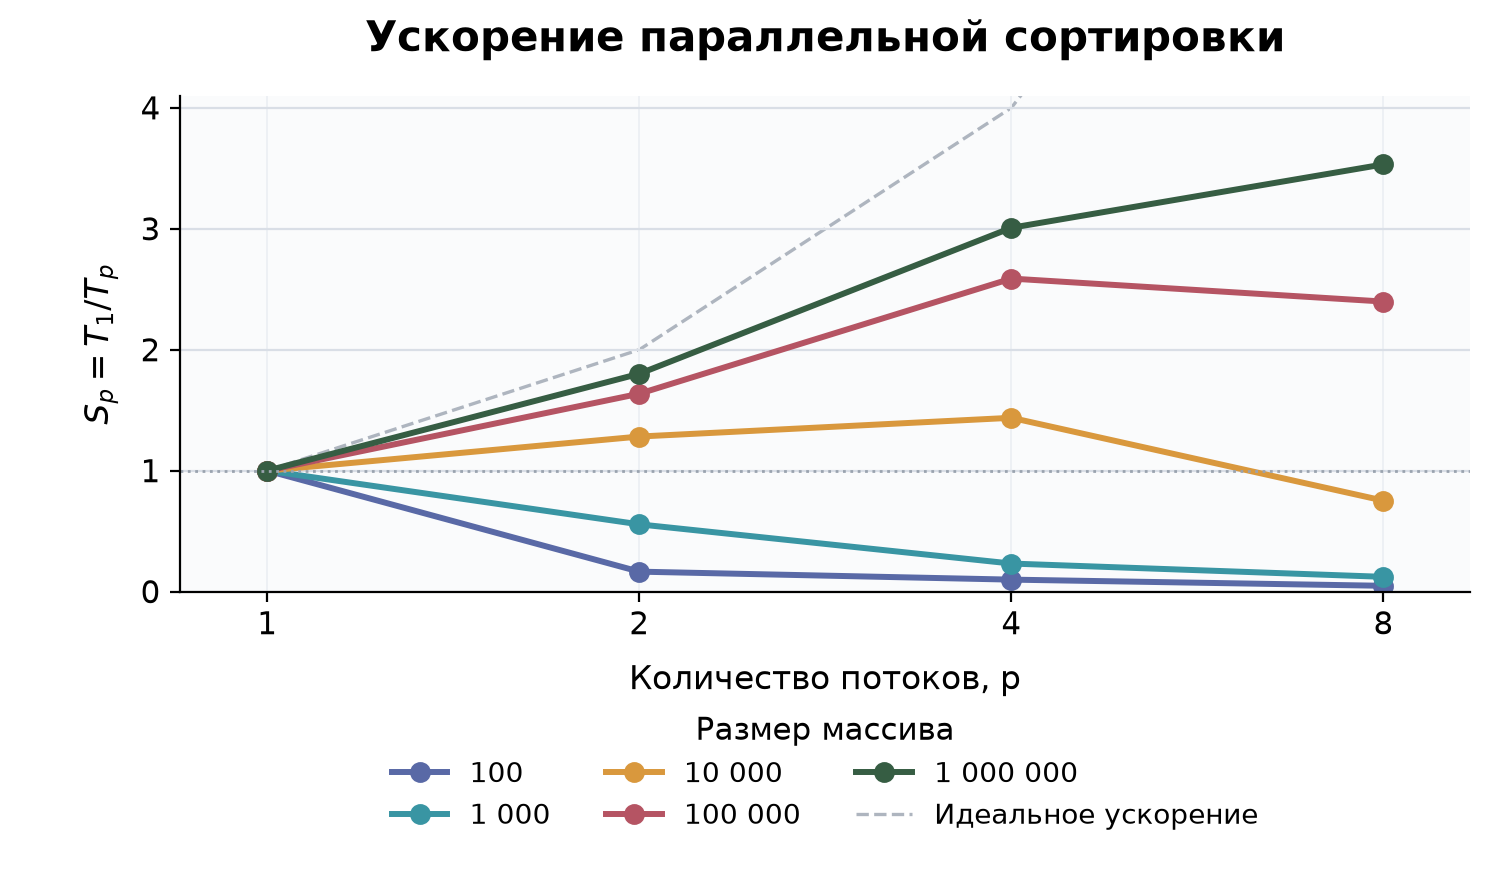
\includegraphics[width=\linewidth]{assets/speedup.png}
  \caption{Зависимость ускорения от числа потоков для пяти входных файлов}
\end{figure}

\begin{figure}[H]
  \centering
  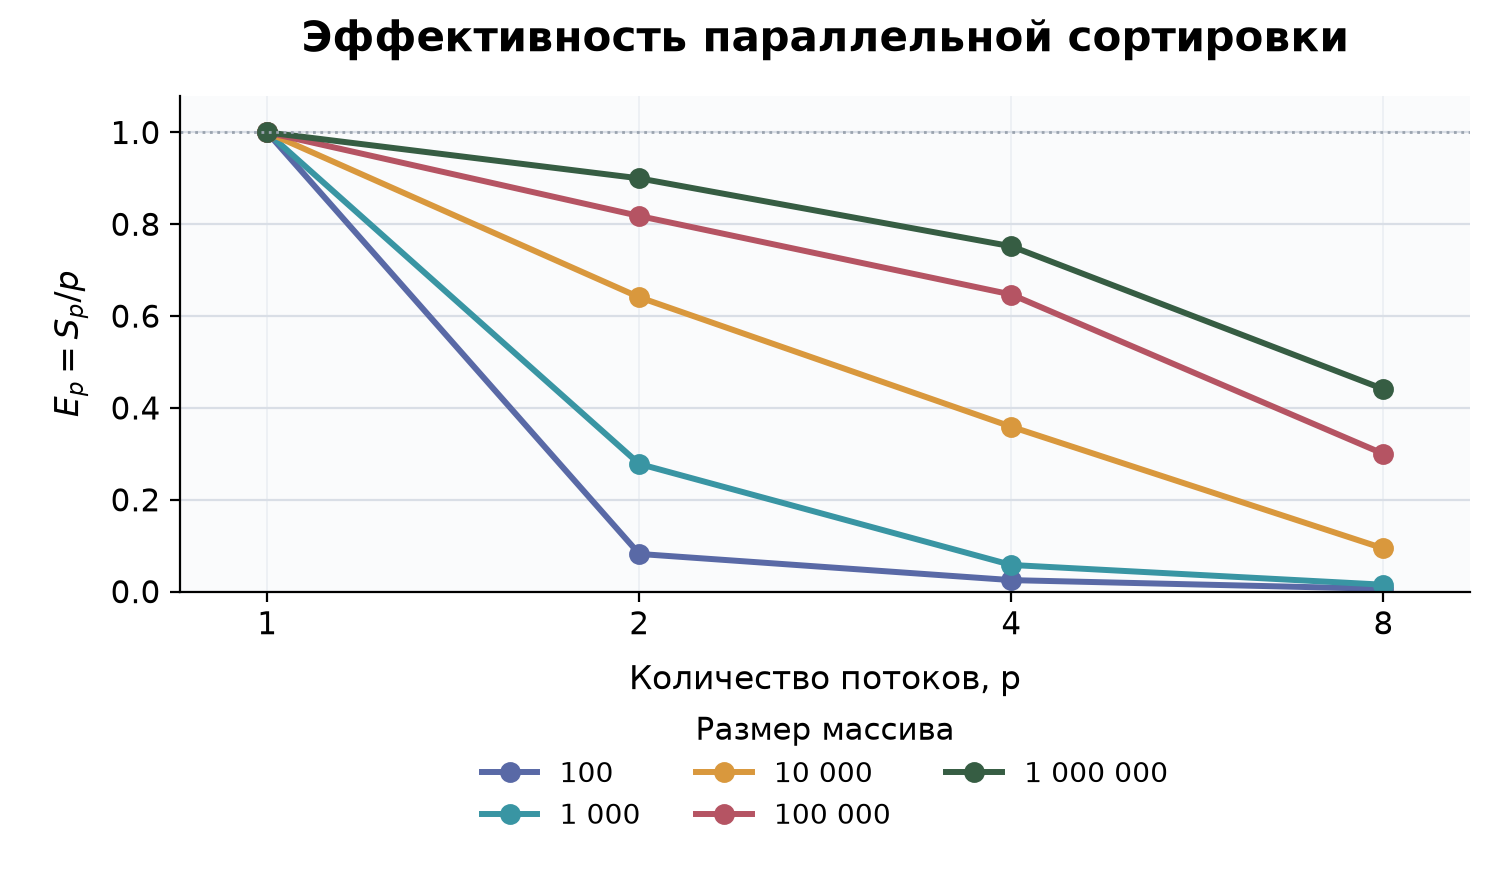
\includegraphics[width=\linewidth]{assets/efficiency.png}
  \caption{Зависимость эффективности от числа потоков для пяти входных файлов}
\end{figure}

На массивах из 100 и 1~000 элементов один поток работает быстрее
нескольких. Для 100 чисел время при одном потоке составило 0.015~мс,
при восьми --- 0.310~мс. Объём полезной
работы мал, а создание потоков и два барьера на каждом проходе требуют
времени. Для файла на 10~000 чисел лучший результат дали четыре потока;
ускорение составило $S_4=1.437$. Для файла на 100~000 чисел тоже лучше
оказались четыре потока: $S_4=2.588$. При восьми потоках на этих размерах
ускорение уменьшается из-за накладных расходов.

На массиве из 1~000~000 элементов время сократилось с 82.537~мс при
одном потоке до 23.370~мс при восьми: $S_8=3.532$, $E_8=0.441$.
Эффективность снижается с ростом числа потоков, поскольку на последних
проходах остаётся мало независимых слияний; потоки ожидают друг друга на
барьерах. На результаты также влияют затраты планировщика и пропускная
способность памяти. Полные численные данные сохранены в
\path{report/measurements.csv} и приведены в приложении Б.

\section{Демонстрация работы strace}

Трассировка получена в Ubuntu ARM64 для файла \path{numbers_10000.txt} с
ключом \texttt{--threads 4}. Команда запуска из корня репозитория:

\begin{terminal}
$ strace -f -o lab_03/report/trace/strace.txt ./build/lab_03/lab3_merge_sort --threads 4 --input lab_03/data/numbers_10000.txt > /dev/null
\end{terminal}

Ниже приведены строки из сокращённой трассировки; полный вывод находится
в \path{report/trace/strace.txt} и приложении В.

\begin{listingblock}{Ключевые системные вызовы из strace}
  \inputterminal{trace/strace_short.txt}
\end{listingblock}

Вызов \texttt{openat()} открывает входной файл, а \texttt{read()} считывает
числа. В трассировке видны три создания потока через \texttt{clone3()}:
главный поток 821490 и дополнительные потоки 821491--821493 вместе дают
четыре потока. Флаги \texttt{CLONE\_VM} и \texttt{CLONE\_THREAD} показывают
общее адресное пространство и принадлежность к одной группе потоков.

Ожидание и пробуждение при работе мьютекса и условной переменной
наблюдаются как вызовы \texttt{futex()}. После завершения дополнительных
потоков главный выводит время и отсортированный массив, затем вызывает
\texttt{exit\_group(0)}. На уровне исходного кода эти действия выполняются
через интерфейсы \texttt{pthread\_*()} и стандартной библиотеки C.

\section{Выводы}

Таким образом, данная лабораторная работа никак кардинально не изменила
мою жизнь: я написал свою первую многопоточную программу и благодаря
лабораторной понял, что можно параллелить разные задачи. Всегда было
интересно, как параллелят разные задачи для алгоритмов машинного обучения
(очень трудно следить, чтобы все потоки правильно отработали, а потом
объединили свои усилия в бОльшую задачу), а тут у самого получилось
написать работающую сортировку. Очень трудоемко.

\appendixsection{А}{Исходный код программы}

\begin{listingblock}{Файл merge\_sort.c}
  \inputappendixcode{../src/merge_sort.c}
\end{listingblock}

\begin{listingblock}{Файл CMakeLists.txt}
  \inputappendixcode{../CMakeLists.txt}
\end{listingblock}

\appendixsection{Б}{Полные результаты измерений}

\begin{listingblock}{Файл measurements.csv}
  \inputterminal{measurements.csv}
\end{listingblock}

\appendixsection{В}{Полный вывод strace}

\begin{listingblock}{Вывод strace -f}
  \inputterminal{trace/strace.txt}
\end{listingblock}

\end{document}
